\documentclass[10pt]{article}

\usepackage{amsmath,amssymb,amsthm}
\usepackage{graphicx}
\usepackage{tikz}

\newtheorem{theorem}{Theorem}
\newtheorem{definition}{Definition}
\newtheorem{lemma}{Lemma}
\newtheorem{example}{Example}
\newtheorem{remark}{Remark}

\newcommand{\defc}{\operatorname{defc}}
\newcommand{\NRCM}{\operatorname{NRCM}}
\newcommand{\clamp}{\operatorname{clamp}}

\title{A Readable Proof of Deficit Preservation for the Naive Rational Cyclic Map}
\author{}
\date{}

\begin{document}

\maketitle

\section{Purpose and setup}

This draft proves that the naive rational cyclic map preserves deficit whenever
the map is defined.  The purpose is readability: the proof is organized around
the few mechanisms that make the theorem true, and examples are included where
they help explain those mechanisms.

Fix coprime positive integers \(r\) and \(s\), and write
\[
  \rho=\frac rs.
\]
Columns are indexed by \(0,1,\ldots,s-1\).  Two background sequences are used
throughout:
\[
  H_i=\left\lfloor\frac{ri}{s}\right\rfloor,
  \qquad
  L_i\equiv ri\pmod s,\qquad 0\le L_i<s.
\]
The number \(H_i\) is the capacity ceiling at column \(i\).  The number
\(L_i\) is the label of column \(i\).  Since \(r\) and \(s\) are coprime, the
labels \(L_0,\ldots,L_{s-1}\) are all distinct.

A rational position-coordinate path is an integer sequence
\[
  Q=(Q_0,\ldots,Q_{s-1})
\]
with
\[
  Q_0=0,\qquad 0\le Q_i\le H_i.
\]
It is often easier to draw the path using the path-height coordinates
\[
  P_i=H_i-Q_i.
\]
We call \(Q\) valid if
\[
  P_0\le P_1\le\cdots\le P_{s-1}.
\]
Thus validity means two things: the coordinates \(Q_i\) fit inside the allowed
capacity \(0\le Q_i\le H_i\), and the path-height sequence \(P_i\) is weakly
increasing.

The deficit formula uses affine heights
\[
  q_i=Q_i+\frac{L_i}{s}.
\]
The capital coordinates \(Q_i\) are integers.  The lowercase coordinates
\(q_i\) remember the same integer data together with the fractional label
order.

\section{Deficit as threshold counts}

For an internal row \(1\le i\le s-2\), define
\[
  C_i(Q)=
  \left[
    -\rho+(q_i-q_{i-1}),\,
    \rho+(q_i-q_{i+1})
  \right].
\]
Because \(P_i=H_i-Q_i\), this same interval is
\[
  C_i(Q)=[P_{i-1}-P_i,\;P_{i+1}-P_i].
\]
For a valid path, both endpoints are integers.  Put
\[
  w_i=P_{i+1}-P_i.
\]
Then
\[
  C_i(Q)=[-w_{i-1},w_i].
\]

For \(1\le i\le s-2\) and \(i<j<s\), set
\[
  \delta_{ij}(Q)=
  \left\lfloor
  \left|
  \clamp_{C_i(Q)}(q_i-q_j)
  \right|
  \right\rfloor,
\]
where \(\clamp_{[a,b]}(x)\) is \(a\) if \(x<a\), is \(x\) if
\(a\le x\le b\), and is \(b\) if \(x>b\).  The row contribution and total
deficit are
\[
  \defc_i(Q)=\sum_{i<j<s}\delta_{ij}(Q),
  \qquad
  \defc(Q)=\sum_{i=1}^{s-2}\defc_i(Q).
\]

The next lemma rewrites each deficit summand as a count of integer thresholds.
This is the form used in the proof: after the NRCM moves values in a suffix,
we compare which thresholds have changed.

\begin{lemma}[Clamp threshold expansion]
Let \(Q\) be valid.  For \(1\le i\le s-2\) and \(i<j<s\),
\[
  \delta_{ij}(Q)=
  \sum_{n=1}^{w_i}{\bf 1}(q_j\le q_i-n)
  +
  \sum_{n=1}^{w_{i-1}}{\bf 1}(q_j\ge q_i+n).
\]
\end{lemma}

\begin{proof}
Since \(C_i(Q)=[-w_{i-1},w_i]\), there are two cases.

If \(q_i>q_j\), then \(q_i-q_j\) is positive and the clamp can only be cut off
at the right endpoint \(w_i\).  The contribution is
\[
  \min\!\left(\left\lfloor q_i-q_j\right\rfloor,w_i\right),
\]
which is the number of integers \(n\) with \(1\le n\le w_i\) and
\[
  q_j\le q_i-n.
\]

If \(q_i<q_j\), the same argument applies at the left endpoint.  The
contribution is the number of integers \(n\) with \(1\le n\le w_{i-1}\) and
\[
  q_j\ge q_i+n.
\]

The equality case \(q_i=q_j\) cannot occur for \(i\ne j\), because the labels
\(L_i\) are distinct.
\end{proof}

\section{The NRCM move}

The map moves a suffix of the \(Q\)-coordinates.  For \(1\le k<s\), let
\[
  I_k=\{k,k+1,\ldots,s-1\}.
\]
The physical suffix \(I_k\) is then ordered by labels.  Write
\[
  \mathcal O_k=(i_1,\ldots,i_{s-k})
\]
for the elements of \(I_k\) listed in increasing order of \(L_i\).

Define \(T_k(Q)\) by moving the \(Q\)-values forward in this label order and
adding \(1\) on the wrap:
\[
  T_k(Q)_{i_{a+1}}=Q_{i_a}\quad(1\le a<s-k),
  \qquad
  T_k(Q)_{i_1}=Q_{i_{s-k}}+1.
\]
Outside the suffix, nothing moves:
\[
  T_k(Q)_j=Q_j\qquad(j\notin I_k).
\]

\begin{definition}[Naive rational cyclic map]
Starting with \(k=1\) and increasing \(k\), choose the first suffix start for
which \(T_k(Q)\) satisfies all capacity conditions
\[
  0\le T_k(Q)_i\le H_i.
\]
If there is no such \(k\), then \(\NRCM(Q)\) is undefined.  If the first
capacity-valid sequence is also valid as a path, define
\[
  \NRCM(Q)=T_k(Q).
\]
Otherwise \(\NRCM(Q)\) is undefined.
\end{definition}

The important point is that the suffix is chosen by capacity first.  The map
does not keep scanning for a later suffix if the first capacity-valid candidate
fails path validity.

\begin{example}[A complete \(36/25\) NRCM step]
For \(r=36\) and \(s=25\), the labels are
\[
  L_i\equiv 36i\equiv 11i\pmod{25}.
\]
Consider
\[
\resizebox{.98\textwidth}{!}{$
Q=(0,0,0,1,0,2,3,3,3,2,2,3,5,6,2,0,2,2,0,0,0,2,2,4,1).
$}
\]
The corresponding path-height sequence is
\[
\resizebox{.98\textwidth}{!}{$
P=(0,1,2,3,5,5,5,7,8,10,12,12,12,12,18,21,21,22,25,27,28,28,29,29,33).
$}
\]
The sequence \(P\) is weakly increasing, so \(Q\) is valid.  The dashed line
marks the first suffix that the NRCM will use.

\[
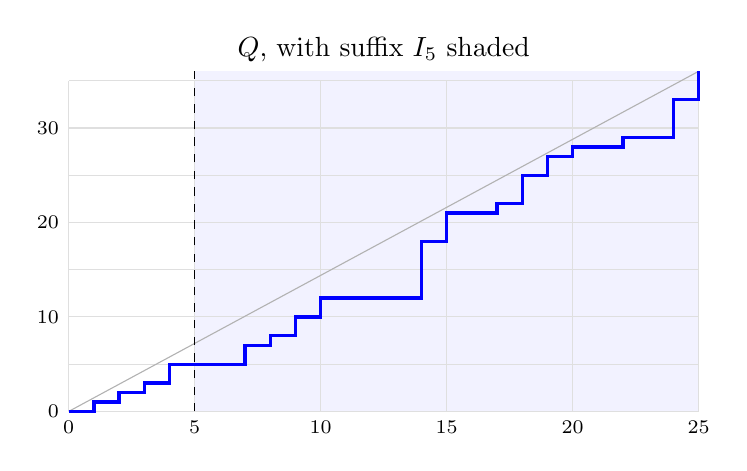
\begin{tikzpicture}[x=.32cm,y=.12cm]
  \fill[blue!5] (5,0) rectangle (25,36);
  \draw[gray!25,step=5] (0,0) grid (25,35);
  \draw[gray!60] (0,0) -- (25,36);
  \draw[dashed] (5,0) -- (5,36);
  \draw[very thick,blue]
    (0,0) -- (1,0) -- (1,1) -- (2,1) -- (2,2) -- (3,2) -- (3,3)
    -- (4,3) -- (4,5) -- (5,5) -- (5,5) -- (6,5) -- (6,5)
    -- (7,5) -- (7,7) -- (8,7) -- (8,8) -- (9,8) -- (9,10)
    -- (10,10) -- (10,12) -- (11,12) -- (11,12) -- (12,12)
    -- (12,12) -- (13,12) -- (13,12) -- (14,12) -- (14,18)
    -- (15,18) -- (15,21) -- (16,21) -- (16,21) -- (17,21)
    -- (17,22) -- (18,22) -- (18,25) -- (19,25) -- (19,27)
    -- (20,27) -- (20,28) -- (21,28) -- (21,28) -- (22,28)
    -- (22,29) -- (23,29) -- (23,29) -- (24,29) -- (24,33)
    -- (25,33) -- (25,36);
  \node[below] at (0,0) {\scriptsize 0};
  \node[below] at (5,0) {\scriptsize 5};
  \node[below] at (10,0) {\scriptsize 10};
  \node[below] at (15,0) {\scriptsize 15};
  \node[below] at (20,0) {\scriptsize 20};
  \node[below] at (25,0) {\scriptsize 25};
  \node[left] at (0,0) {\scriptsize 0};
  \node[left] at (0,10) {\scriptsize 10};
  \node[left] at (0,20) {\scriptsize 20};
  \node[left] at (0,30) {\scriptsize 30};
  \node[above] at (12.5,36) {\(Q\), with suffix \(I_5\) shaded};
\end{tikzpicture}
\]

For \(k=1,2,3,4\), the suffix candidate fails capacity; the first failing
column is respectively \(1,2,3,4\).  The first capacity-valid suffix is
\[
  I_5=\{5,6,\ldots,24\}.
\]
In increasing label order this suffix is
\[
\resizebox{.98\textwidth}{!}{$
\mathcal O_5=(16,7,23,14,5,21,12,19,10,17,8,24,15,6,22,13,20,11,18,9).
$}
\]
Thus the value at \(16\) moves to \(7\), the value at \(7\) moves to \(23\),
and so on, with the value at \(9\) returning to \(16\) after adding \(1\).
This gives
\[
\resizebox{.98\textwidth}{!}{$
Q'=(0,0,0,1,0,2,0,2,2,0,0,0,2,2,4,1,3,2,3,5,6,2,3,3,3).
$}
\]
The image path-height sequence is
\[
\resizebox{.98\textwidth}{!}{$
P'=(0,1,2,3,5,5,8,8,9,12,14,15,15,16,16,20,20,22,22,22,22,28,28,30,31).
$}
\]
It is again valid.

\[
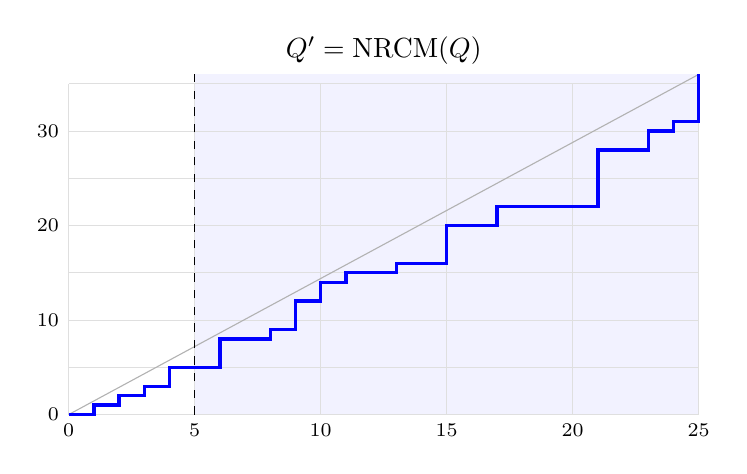
\begin{tikzpicture}[x=.32cm,y=.12cm]
  \fill[blue!5] (5,0) rectangle (25,36);
  \draw[gray!25,step=5] (0,0) grid (25,35);
  \draw[gray!60] (0,0) -- (25,36);
  \draw[dashed] (5,0) -- (5,36);
  \draw[very thick,blue]
    (0,0) -- (1,0) -- (1,1) -- (2,1) -- (2,2) -- (3,2) -- (3,3)
    -- (4,3) -- (4,5) -- (5,5) -- (5,5) -- (6,5) -- (6,8)
    -- (7,8) -- (7,8) -- (8,8) -- (8,9) -- (9,9) -- (9,12)
    -- (10,12) -- (10,14) -- (11,14) -- (11,15) -- (12,15)
    -- (12,15) -- (13,15) -- (13,16) -- (14,16) -- (14,16)
    -- (15,16) -- (15,20) -- (16,20) -- (16,20) -- (17,20)
    -- (17,22) -- (18,22) -- (18,22) -- (19,22) -- (19,22)
    -- (20,22) -- (20,22) -- (21,22) -- (21,28) -- (22,28)
    -- (22,28) -- (23,28) -- (23,30) -- (24,30) -- (24,31)
    -- (25,31) -- (25,36);
  \node[below] at (0,0) {\scriptsize 0};
  \node[below] at (5,0) {\scriptsize 5};
  \node[below] at (10,0) {\scriptsize 10};
  \node[below] at (15,0) {\scriptsize 15};
  \node[below] at (20,0) {\scriptsize 20};
  \node[below] at (25,0) {\scriptsize 25};
  \node[left] at (0,0) {\scriptsize 0};
  \node[left] at (0,10) {\scriptsize 10};
  \node[left] at (0,20) {\scriptsize 20};
  \node[left] at (0,30) {\scriptsize 30};
  \node[above] at (12.5,36) {\(Q'=\NRCM(Q)\)};
\end{tikzpicture}
\]

For this example,
\[
  \defc(Q)=214=\defc(Q').
\]
The theorem will prove that this equality holds for every \(Q\) for which
\(\NRCM(Q)\) is defined.
\end{example}

\section{Suffix label geometry and omitted-column fit}

For the rest of the proof, fix a valid path \(Q\), assume
\[
  Q'=\NRCM(Q)
\]
is defined, and let \(K=I_k\) be the suffix chosen by the NRCM.  If \(k>1\),
write
\[
  b=k-1
\]
for the boundary column immediately before the moved suffix.

If \(a\in K\), write \(\operatorname{pred}_K(a)\) and
\(\operatorname{succ}_K(a)\) for the previous and next elements of \(K\) in
increasing label order, cyclically.  For any two columns \(a,c\), set
\[
  \epsilon(a,c)={\bf 1}_{L_c<L_a}.
\]
This records whether the label step from \(a\) to \(c\) wraps around the end
of the label order.  Thus the value at \(a\in K\) moves to
\(\operatorname{succ}_K(a)\) as
\[
  Q_a+\epsilon(a,\operatorname{succ}_K(a)).
\]

Now let \(0<h<k\) be an omitted column.  Column \(0\) is fixed at \(Q_0=0\)
and is not an internal deficit row, so the omitted-column fit notation is only
needed for \(0<h<k\).  Insert \(h\) into the cyclic label order on \(K\).  Let
\[
  \alpha_h\in K,\qquad \beta_h\in K
\]
be the predecessor and successor of \(h\) in this enlarged order.  Define
\[
  \epsilon_h=\epsilon(\alpha_h,h),
  \qquad
  \mu_h=H_h-Q_{\alpha_h}-\epsilon_h.
\]
The number \(Q_{\alpha_h}+\epsilon_h\) is the coordinate that would be sent to
the omitted column \(h\) if \(h\) were added to the moved suffix.  The
quantity \(\mu_h\) is the remaining capacity at \(h\) for that hypothetical
incoming value.  Thus \(\mu_h<0\) means the value would not fit at \(h\).

\begin{example}[The omitted-column data in the \(36/25\) move]
For the \(36/25\) example above, the selected suffix is \(K=I_5\), so the
omitted columns are \(1,2,3,4\).  The omitted-column data generated from the
example is
\[
\begin{array}{c|c|c|c|c}
h & \alpha_h & \beta_h & \epsilon_h & \mu_h\\ \hline
1 & 10 & 17 & 0 & -1\\
2 & 11 & 18 & 0 & -1\\
3 & 12 & 19 & 0 & -2\\
4 & 13 & 20 & 0 & -1
\end{array}
\]
Every \(\mu_h\) is negative, so each omitted column would overflow if it were
added to the selected suffix.  This is the example version of the omitted-edge
overflow lemma proved below.
\end{example}

\subsection*{A noncrossing fact for the suffix cycle}

The next lemma does not use the path \(Q\).  It only concerns the label cycle
on the selected suffix \(K\).  When the boundary column \(b=k-1\) is inserted
into that label cycle, the wrap edge is
\[
  \alpha_b\to\beta_b.
\]
The lemma says that no ordinary edge of the suffix cycle crosses this wrap
edge in physical order.

\begin{example}[A \(7/17\) residue table]
Take \(r=7\), \(s=17\), and suppose the suffix starts at \(k=6\).  Then the
boundary column is \(b=k-1=5\), and the suffix is \(K=\{6,\ldots,16\}\).
The full residue table is
\[
\resizebox{.98\textwidth}{!}{$
\begin{array}{c|ccccccccccccccccc}
x&0&1&2&3&4&5&6&7&8&9&10&11&12&13&14&15&16\\ \hline
7x\bmod17&0&7&14&4&11&1&8&15&5&12&2&9&16&6&13&3&10
\end{array}
$}
\]
From the boundary column \(b=5\), a suffix column \(x\in K\) is recorded by
its gap
\[
  g=x-b.
\]
Thus \(N=s-k=11\), and the relevant gaps are \(g=1,\ldots,11\), corresponding
to physical columns \(x=6,\ldots,16\).  Their residues relative to \(b\) are
\[
\begin{array}{c|ccccccccccc}
g&1&2&3&4&5&6&7&8&9&10&11\\ \hline
7g\bmod17&7&14&4&11&1&8&15&5&12&2&9
\end{array}
\]
Sorting the gaps by residue gives
\[
  (5,10,3,8,1,6,11,4,9,2,7).
\]
Adding \(b=5\) to each gap converts this into the suffix columns in label order:
\[
  (10,15,8,13,6,11,16,9,14,7,12).
\]
Since \(L_b=1\), inserting \(b=5\) puts it just before the column \(10\).  Thus
\[
  \beta_b=10,\qquad \alpha_b=12,
\]
and the wrap edge in the suffix cycle is \(12\to10\).  The lemma says that an
ordinary suffix-cycle edge whose target lies to the right of \(10\) must have
source to the left of \(12\).  For example, \(6\to11\) is allowed because
\(6<12\), while an edge such as \(14\to13\) would be forbidden.
\end{example}

\begin{lemma}[Suffix-cycle noncrossing]
Let \(b=k-1\) and \(K=I_k\).  Let \(\operatorname{succ}_K\) be successor in
the label cycle on \(K\).  If \(a\in K\) and \(a>\alpha_b\), then
\[
  \operatorname{succ}_K(a)<\beta_b.
\]
Equivalently, every ordinary suffix-cycle edge whose source is physically to
the right of \(\alpha_b\) has target physically to the left of \(\beta_b\).
\end{lemma}

\begin{proof}
Put \(N=s-k\).  For any integer column position \(x\), let
\[
  R(x)\equiv L_x-L_b\pmod s,\qquad 0\le R(x)<s.
\]
Thus \(R(x)\) is the label of \(x\), measured relative to the label of \(b\).
Since \(\beta_b\) is the first suffix column after \(b\) in label order and
\(\alpha_b\) is the last one before \(b\), they have the smallest and largest
relative labels among suffix columns:
\[
  R(\beta_b)\le R(x)\le R(\alpha_b).
\]
The inequalities are strict when \(x\ne\beta_b,\alpha_b\).

Suppose, toward a contradiction, that an ordinary suffix-cycle edge
\[
  a\to c=\operatorname{succ}_K(a)
\]
has
\[
  a>\alpha_b,\qquad c\ge\beta_b.
\]
The first inequality says \(a-b>\alpha_b-b\).  Also
\(c-b\ne\beta_b-b\), because \(\beta_b\) is the target of the wrap edge
\(\alpha_b\to\beta_b\), not the target of an ordinary edge.  Hence
\[
  c-b>\beta_b-b.
\]
The edge \(a\to c\) is ordinary in label order, so
\[
  R(a)<R(c)
\]
and there is no suffix column whose relative label lies strictly between
\(R(a)\) and \(R(c)\).

First note that \((\beta_b-b)+(\alpha_b-b)>N\).  If
\((\beta_b-b)+(\alpha_b-b)\le N\), then
\[
  R(\beta_b+\alpha_b-b)
  \equiv
  R(\beta_b)+R(\alpha_b)\pmod s.
\]
This residue is either larger than the maximum suffix residue
\(R(\alpha_b)\), smaller than the minimum suffix residue \(R(\beta_b)\),
or equal to \(0\).  Each case is impossible.

Now put
\[
  d=R(c)-R(a)>0.
\]
We claim \(d>R(\beta_b)\).  Suppose \(d\le R(\beta_b)\).  If \(c>a\), set
\[
  n=c-a.
\]
Then \(1\le n<\beta_b-b\), because \(a-b>\alpha_b-b\) and
\((\beta_b-b)+(\alpha_b-b)>N\).  But then
\[
  R(b+n)=d\le R(\beta_b),
\]
contradicting the minimality of \(R(\beta_b)\) among suffix columns.

If \(c<a\), set \(n=a-c\).  Since \(c>\beta_b\), the column
\(\beta_b+n=\beta_b+a-c\) still lies in \(K\).  Also
\[
  R(\beta_b+n)\equiv R(\beta_b)-d\pmod s.
\]
If \(d<R(\beta_b)\), this is a positive residue smaller than \(R(\beta_b)\);
if \(d=R(\beta_b)\), it is \(0\).  Both are impossible.  Hence
\(d>R(\beta_b)\).

Finally, because \(c>\beta_b\), the column
\[
  z=b+c-\beta_b
\]
belongs to \(K\), and
\[
  R(z)=R(c)-R(\beta_b).
\]
Since \(d=R(c)-R(a)>R(\beta_b)\), we have
\[
  R(a)<R(c)-R(\beta_b)<R(c).
\]
Thus \(z\) gives a suffix column whose relative label lies strictly between
\(R(a)\) and \(R(c)\),
contradicting that \(a\to c\) is an ordinary edge in the label cycle.
\end{proof}

\subsection*{Comparing omitted columns}

For an omitted column \(t<k\), the gap from \(t\) to \(\beta_t\) is
\[
  g_t=\beta_t-t.
\]
This gap can also be read as the position of \(\beta_t\) after shifting the
suffix \(K\) left by \(t\).  The next lemma says that earlier omitted columns
see their first suffix column at least as far to the right as the boundary
column does.

\begin{lemma}[Successor-gap dominance]
Let \(k>1\), let \(b=k-1\), and let \(0<t<k\).  Then \(g_t\) is the unique
minimizer of \(rg\pmod s\) on
\[
  [k-t,s-1-t].
\]
In particular, for every \(0<i<b\),
\[
  g_i\ge g_b=\beta_b-b.
\]
\end{lemma}

\begin{proof}
For \(g\in[k-t,s-1-t]\), the column \(t+g\) runs through \(K\).  The cyclic
label increment from \(t\) to \(t+g\) is \(rg\pmod s\), so \(\beta_t\) is the
suffix column whose shifted position \(g_t\) has the smallest positive label
increment.

For \(b=k-1\), the shifted interval is \([1,s-k]\).  Put \(d=b-i>0\).  For
\(i\), the shifted interval is
\[
  [k-i,s-1-i]=[d+1,s-k+d].
\]
Let \(f=g_b\), the minimum-position in the boundary interval.  If \(f<d+1\),
then every position in the shifted interval for \(i\) lies to the right of
\(f\), so \(g_i>f\).  Otherwise \(f\) belongs to the shifted interval for
\(i\).  No position to the left of \(f\) in that interval can have smaller
label, because those positions also occur in the boundary interval, where
\(f\) is minimal.  Hence \(g_i\) is either \(f\) or lies to its right.
\end{proof}

\begin{example}[The hard shifted-window case in \(13/10\)]
For \(r=13\), \(s=10\), take
\[
  Q=(0,1,2,3,5,6,7,6,7,8).
\]
The NRCM chooses \(k=7\), so \(b=6\) and
\[
  K=\{7,8,9\},\qquad \mathcal O_7=(7,8,9).
\]
The labels are
\[
  L=(0,3,6,9,2,5,8,1,4,7).
\]
For the boundary column, \(\beta_b=7\) and \(\alpha_b=9\).  Several earlier
omitted columns have \(\beta_i>\beta_b\):
\[
\begin{array}{c|c|c|c|c}
i&\beta_i&\alpha_i&\beta_b&\alpha_b\\ \hline
1&8&7&7&9\\
2&9&8&7&9\\
4&8&7&7&9\\
5&9&8&7&9
\end{array}
\]
For \(i=5\), the conclusion below reads
\[
  5<6<8<9,\qquad 0<9-8\le6-5,\qquad L_8<L_5.
\]
Indeed, \(L_8=4<L_5=5\).
\end{example}

\begin{lemma}[Shifted suffix-window facts]
Let \(b=k-1\), and let \(0<i<b\).  If \(\beta_i>\beta_b\), then
\[
  0<\alpha_b-\alpha_i\le b-i,\qquad
  L_{\alpha_i}<L_i.
\]
\end{lemma}

\begin{proof}
Put \(N=s-k\) and \(d=b-i\).  Use the same relative-label convention as above:
for any integer column position \(x\), let
\[
  R(x)\equiv L_x-L_b\pmod s,\qquad 0\le R(x)<s.
\]
Thus \(\beta_b\) is the suffix column with smallest \(R\)-value, and
\(\alpha_b\) is the suffix column with largest \(R\)-value.

From the viewpoint of \(i=b-d\), a suffix column \(x\in K\) has relative label
\[
  R(x+d)\equiv L_x-L_i\pmod s.
\]
Thus the order seen from \(i\) is obtained from the order seen from \(b\) by
adding the same label increment to every suffix column.  The column \(\beta_i\)
is the minimum in this shifted order, and \(\alpha_i\) is its predecessor.

By the contrapositive of suffix-cycle noncrossing, an ordinary edge landing to
the right of \(\beta_b\) cannot have source at or to the right of
\(\alpha_b\).  Applying this to the edge \(\alpha_i\to\beta_i\) gives
\[
  \alpha_i<\alpha_b.
\]

We now show that \(\alpha_i\) is not too far left of \(\alpha_b\).  Suppose
\[
  \alpha_i+d<\alpha_b.
\]
Then \(\alpha_i+d\) is a suffix column, so maximality of \(\alpha_b\) in the
boundary order gives
\[
  R(\alpha_b)>R(\alpha_i+d).
\]
Also \(\alpha_b-d\) is a suffix column, because the assumption is equivalent to
\(\alpha_i<\alpha_b-d\).  Since \(\alpha_i\) is the maximum in the shifted
order, applied to the suffix column \(\alpha_b-d\), we get
\[
  R(\alpha_i+d)>R((\alpha_b-d)+d)=R(\alpha_b).
\]
This contradicts the previous display.  Hence
\[
  \alpha_b\le\alpha_i+d,
\]
and therefore
\[
  0<\alpha_b-\alpha_i\le d=b-i.
\]

  Finally, translating columns by \(d=b-i\) moves the viewpoint from \(i\) to
\(b\).  Thus \(\alpha_i+d\) is the column whose distance from \(b\) is the
same as the distance from \(i\) to \(\alpha_i\):
\[
  (\alpha_i+d)-b=\alpha_i-i.
\]
Since \(\alpha_i\) is the predecessor of the shifted minimum,
it is on the wrapped side of the shifted cut, so
\[
  L_i+R(\alpha_i+d)\ge s.
\]
Since \(R(\alpha_i+d)\equiv L_{\alpha_i}-L_i\pmod s\), we get
\[
  L_{\alpha_i}=L_i+R(\alpha_i+d)-s<L_i.
\]
\end{proof}

\subsection*{Omitted-column fit bounds}

The next lemmas turn the label geometry into a capacity statement.  The goal
is to prove that every omitted column would overflow if it were inserted into
the chosen suffix.  This is the reason the NRCM chose \(K\) rather than an
earlier suffix.

\begin{lemma}[Projection identity for omitted-column fit]
Let \(Q'=T_k(Q)\).  For \(0<t<k\),
\[
  \mu_t
  =
  P'_{\beta_t}
  -
  \left\lfloor\frac{r(\beta_t-t)}s\right\rfloor .
\]
\end{lemma}

\begin{proof}
If the omitted column \(t\) were inserted into the label cycle on \(K\), the
incoming value at \(t\) would come from \(\alpha_t\), and the next target would
be \(\beta_t\).  In the actual \(K\)-move this value lands at \(\beta_t\), so
\[
  P'_{\beta_t}
  =
  H_{\beta_t}-Q_{\alpha_t}-\epsilon(\alpha_t,\beta_t).
\]
The label step \(\alpha_t\to\beta_t\) factors through \(t\).  Therefore
\[
  \epsilon(\alpha_t,\beta_t)
  =
  \epsilon(\alpha_t,t)+\epsilon(t,\beta_t).
\]
Also
\[
  H_{\beta_t}-H_t
  =
  \left\lfloor\frac{r(\beta_t-t)}s\right\rfloor
  +
  \epsilon(t,\beta_t).
\]
Substituting these two identities into the display for \(P'_{\beta_t}\) gives
the claimed formula for \(\mu_t=H_t-Q_{\alpha_t}-\epsilon(\alpha_t,t)\).
\end{proof}

\begin{lemma}[Hard-case lift inequality]
Let \(i<b<\alpha<A\).  Suppose
\[
  0<A-\alpha\le b-i,\qquad L_\alpha<L_i.
\]
Then
\[
  H_A-H_\alpha-\epsilon(\alpha,i)+\epsilon(A,b)\le H_b-H_i.
\]
\end{lemma}

\begin{proof}
The floor parts are monotone because \(A-\alpha\le b-i\).  The only possible
loss comes from the wrap indicators, so the proof checks those wrap cases.

Since \(L_\alpha<L_i\), we have \(\epsilon(\alpha,i)=0\).  Put
\[
  d_0=A-\alpha,\qquad d=b-i,
\]
and write
\[
  rd_0=us+\theta,\qquad rd=vs+\sigma,\qquad 0\le\theta,\sigma<s.
\]
Because \(d_0\le d\), either \(u<v\), or \(u=v\) and \(\theta\le\sigma\).
Using
\[
  H_y-H_x=\left\lfloor\frac{r(y-x)}s\right\rfloor+\epsilon(x,y),
\]
it remains to prove
\[
  u+\epsilon(\alpha,A)+\epsilon(A,b)\le v+\epsilon(i,b).
\]
If \(u\le v-2\), this is immediate.  If \(u=v-1\), the only dangerous case is
\(\epsilon(\alpha,A)=\epsilon(A,b)=1\) and \(\epsilon(i,b)=0\).  But then
\[
  L_A<L_\alpha<L_i,\qquad L_b<L_A,
\]
so \(L_b<L_i\), contradicting \(\epsilon(i,b)=0\).

Now suppose \(u=v\).

If \(\epsilon(\alpha,A)=1\), then \(L_\alpha+\theta\ge s\).  Since
\(L_i>L_\alpha\) and \(\theta\le\sigma\), we get \(\epsilon(i,b)=1\).  Also
\[
  L_A=L_\alpha+\theta-s<L_i+\sigma-s=L_b,
\]
so \(\epsilon(A,b)=0\).

If \(\epsilon(\alpha,A)=0\), then \(\epsilon(A,b)=1\) forces
\(\epsilon(i,b)=1\); otherwise
\[
  L_b=L_i+\sigma>L_\alpha+\theta=L_A,
\]
a contradiction.
\end{proof}

\begin{lemma}[Rightmost omitted-column fit dominance]
Assume \(Q\) and \(Q'=T_k(Q)\) are valid.  If \(k>1\), then
\[
  \mu_i\le \mu_{k-1}\qquad(0<i<k).
\]
\end{lemma}

\begin{proof}
Put \(b=k-1\).  By the projection identity,
\[
  \mu_t
  =
  P'_{\beta_t}
  -
  \left\lfloor\frac{r(\beta_t-t)}s\right\rfloor .
\]
If \(\beta_i\le\beta_b\), validity of \(Q'\) gives
\[
  P'_{\beta_i}\le P'_{\beta_b},
\]
and successor-gap dominance gives
\[
  \left\lfloor\frac{r(\beta_i-i)}s\right\rfloor
  \ge
  \left\lfloor\frac{r(\beta_b-b)}s\right\rfloor .
\]
Hence \(\mu_i\le\mu_b\).

Now suppose \(\beta_i>\beta_b\).  By the shifted suffix-window facts,
\[
  0<\alpha_b-\alpha_i\le b-i,\qquad
  L_{\alpha_i}<L_i.
\]
Since \(\alpha_i,\alpha_b\in K\) and \(i<b\), this also gives
\[
  i<b<\alpha_i<\alpha_b.
\]
Validity of \(Q\) gives
\[
  Q_{\alpha_b}-Q_{\alpha_i}\le H_{\alpha_b}-H_{\alpha_i}.
\]
Therefore
\[
  \begin{aligned}
  \mu_i-\mu_b
  &=H_i-H_b+Q_{\alpha_b}-Q_{\alpha_i}
    -\epsilon(\alpha_i,i)+\epsilon(\alpha_b,b)\\
  &\le H_i-H_b+H_{\alpha_b}-H_{\alpha_i}
    -\epsilon(\alpha_i,i)+\epsilon(\alpha_b,b)\\
  &\le0
  \end{aligned}
\]
by the hard-case lift inequality.
\end{proof}

\begin{lemma}[Omitted-edge overflow]
Let \(Q'=\NRCM(Q)\), and let \(K=I_k\) be the suffix selected by the NRCM.
For every omitted column \(0<h<k\),
\[
  Q_{\alpha_h}+\epsilon_h>H_h.
\]
\end{lemma}

\begin{proof}
If \(k=1\), there are no omitted columns.  Suppose \(k>1\), and put
\(b=k-1\).

Assume some omitted column \(0<h<k\) does not overflow.  Then \(\mu_h\ge0\).
By rightmost omitted-column fit dominance, \(\mu_b\ge0\).  Hence the incoming
value from \(\alpha_b\) would fit at \(b\):
\[
  Q_{\alpha_b}+\epsilon(\alpha_b,b)\le H_b.
\]

Now compare the chosen suffix \(K=I_k\) with the earlier suffix
\[
  I_{k-1}=\{b\}\cup K.
\]
Inserting \(b\) into the label cycle on \(K\) changes only two targets: the
old target \(\beta_b\), and the new target \(b\).  The new target \(b\) fits
by the previous display.  The old value at \(b\) also fits at \(\beta_b\),
because \(Q\) itself is valid and
\[
  Q_b+\epsilon(b,\beta_b)\le H_{\beta_b}.
\]
All other target columns receive the same values as in the capacity-valid
\(K\)-candidate.  Thus \(I_{k-1}\) would have been capacity-valid, contradicting
the choice of \(K=I_k\) as the first capacity-valid suffix.
\end{proof}

\section{Prefix rows}

The deficit is a sum over rows.  The rows before the boundary row are the
prefix rows
\[
  1,\ldots,k-2.
\]
For such a row \(i\), the row itself and its neighbors \(i-1,i+1\) are outside
the moved suffix.  Therefore the base point \(q_i\) and the clamp interval
\[
  C_i(Q)=[-w_{i-1},w_i]
\]
do not move.  Only the comparisons with suffix columns \(j\in K\) can change.

The next lemma says that after we index the moved suffix values by their source
columns, every source cancels except the one whose label arc crosses the
omitted row \(i\).  That source is \(\alpha_i\), the predecessor of \(i\) when
\(i\) is inserted into the suffix label order.

\begin{lemma}[Threshold crossing for an omitted row]
Fix an internal omitted row \(1\le i\le k-2\).  Reindex the after-sum over
suffix targets by their source columns in \(K\).  All changing terms in
\(\defc_i\) cancel except the possible crossing at \(\alpha_i\).  If
\[
  m_i=Q_{\alpha_i}+\epsilon_i-Q_i,
\]
then the total change in the terms of \(\defc_i\) with second index in \(K\)
is
\[
  {\bf 1}(1\le m_i\le w_{i-1})
  -
  {\bf 1}(-w_i\le m_i\le -1).
\]
\end{lemma}

\begin{proof}
Since \(i\le k-2\), the row \(i\) and its neighbors are outside the moved
suffix.  Hence \(q_i\) and \(C_i(Q)=[-w_{i-1},w_i]\) are unchanged.

Let \(\sigma=\operatorname{succ}_K\).  The value originally at \(a\in K\)
lands at \(\sigma(a)\), with
\[
  q'_{\sigma(a)}
  =
  Q_a+\epsilon(a,\sigma(a))+\frac{L_{\sigma(a)}}s.
\]
So the label part of \(q_a\) moves along the lifted interval
\[
  A_a=[L_a,\ L_{\sigma(a)}+s\epsilon(a,\sigma(a))).
\]
As \(a\) runs through \(K\), these half-open intervals are consecutive and
disjoint, and together they make one full turn of length \(s\).  Therefore
exactly one of them contains the lifted label of \(i\).  Its source is
\(\alpha_i\).

If \(a\ne\alpha_i\), then \(q_a\) and the transported point
\(q'_{\sigma(a)}\) stay on the same side of every integer threshold
\[
  q_i+c,\qquad c\in\mathbb Z.
\]
The integer coordinate of the transported source changes only by the wrap
already recorded in the lifted label interval \(A_a\), so crossing an integer
threshold is equivalent to that lifted interval containing the label of \(i\).
Thus source \(a\) contributes no change to any threshold count.

For an integer \(c\), set
\[
  D_i(c)=
  \sum_{a\in K}
  \left(
    {\bf 1}(q'_{\sigma(a)}\le q_i+c)
    -
    {\bf 1}(q_a\le q_i+c)
  \right).
\]
Only \(a=\alpha_i\) can contribute to \(D_i(c)\).  On that arc, the threshold
\(q_i+c\) is crossed exactly when
\[
  Q_i+c=Q_{\alpha_i}+\epsilon_i,
\]
or \(c=m_i\).  With the half-open convention, the old point is counted and the
new transported point is not counted in this case.  Hence
\[
  D_i(c)=-{\bf 1}(c=m_i).
\]

Apply the clamp threshold expansion.  The lower thresholds contribute
\[
\begin{aligned}
&\sum_{j=k}^{s-1}
\sum_{n=1}^{w_i}
\left(
  {\bf 1}(q'_j\le q_i-n)
  -
  {\bf 1}(q_j\le q_i-n)
\right)\\
&\qquad=
\sum_{n=1}^{w_i}D_i(-n)
=
-{\bf 1}(-w_i\le m_i\le -1).
\end{aligned}
\]
For upper thresholds, no target level equals \(q_i+n\), since the residues are
distinct.  Therefore the change in the number of targets above \(q_i+n\) is
the negative of the change in the number below \(q_i+n\):
\[
\begin{aligned}
&\sum_{j=k}^{s-1}
\sum_{n=1}^{w_{i-1}}
\left(
  {\bf 1}(q'_j\ge q_i+n)
  -
  {\bf 1}(q_j\ge q_i+n)
\right)\\
&\qquad=
-\sum_{n=1}^{w_{i-1}}D_i(n)
=
{\bf 1}(1\le m_i\le w_{i-1}).
\end{aligned}
\]
Adding the lower and upper parts gives the stated identity.
\end{proof}

\begin{example}[Prefix rows in the \(36/25\) move]
In the \(36/25\) example, \(k=5\), so the prefix rows are \(1,2,3\).  The
verified omitted-column data gives
\[
\begin{array}{c|c|c|c|c|c}
i & \alpha_i & \epsilon_i & \mu_i & m_i & (w_{i-1},w_i)\\ \hline
1 & 10 & 0 & -1 & 2 & (1,1)\\
2 & 11 & 0 & -1 & 3 & (1,1)\\
3 & 12 & 0 & -2 & 4 & (1,2)
\end{array}
\]
For each prefix row, \(m_i\) is larger than the upper threshold range
\([1,w_{i-1}]\) and is not in the lower range \([-w_i,-1]\).  Thus the
possible crossing contributes zero to the total row change.
\end{example}

\begin{lemma}[Prefix rows do not change]
Let \(Q'=\NRCM(Q)\), and let \(K=I_k\) be the suffix selected by the NRCM.
For every internal row \(1\le i\le k-2\),
\[
  \defc_i(Q')=\defc_i(Q).
\]
\end{lemma}

\begin{proof}
For \(1\le i\le k-2\), the row \(i\) and its two neighbors \(i-1,i+1\) are
outside the moved suffix.  Hence \(q_i\), \(C_i(Q)\), and the pair terms
\(\delta_{ij}\) with \(j<k\) are unchanged.

It remains to compare the terms with \(j\in K\).  By the threshold-crossing
lemma, their total change is
\[
  {\bf 1}(1\le m_i\le w_{i-1})
  -
  {\bf 1}(-w_i\le m_i\le -1),
  \qquad
  m_i=Q_{\alpha_i}+\epsilon_i-Q_i.
\]
By omitted-edge overflow,
\[
  Q_{\alpha_i}+\epsilon_i>H_i.
\]
Therefore
\[
  m_i>H_i-Q_i=P_i.
\]
Since
\[
  w_{i-1}=P_i-P_{i-1}\le P_i,
  \qquad
  w_i\ge0,
\]
the integer \(m_i\) lies in neither threshold range.  Both indicators are
zero, and hence \(\defc_i(Q')=\defc_i(Q)\).
\end{proof}

\begin{remark}
The boundary row \(k-1\) is not a prefix row for this argument.  Its right
neighbor is inside the moved suffix, so its clamp interval changes.  The
boundary row is handled together with the rows inside the suffix.
\end{remark}

\section{Boundary and suffix rows}

The prefix rows are done.  The only remaining deficit terms are the boundary
row \(b=k-1\), if \(b>0\), and the rows inside the moved suffix \(K\).  These
rows are harder because the physical slack intervals
\[
  (P_e,P_{e+1})
\]
may change when the suffix values move.

The proof below reorganizes the clamp-threshold counts by physical edge.  The
resulting objects are signed endpoints on those physical edges.  Endpoints
inside the visible edge list pair with opposite signs.  The only possible
unpaired endpoints would sit next to omitted columns, and omitted-edge overflow
rules those out.

In the two abstract endpoint lemmas below, ``deleted'' means that an endpoint
or cut is not part of the visible list being paired.  In the later physical-edge
application, the deleted cuts are exactly the cuts next to omitted columns.

For a finite signed multiset \(\mathcal T\), write
\[
  \omega(\mathcal T)=\sum_{\tau\in\mathcal T}\operatorname{sgn}(\tau),
\]
with multiplicity.

\begin{lemma}[Label-order endpoint cancellation]
Let \(\mathcal I\) be a finite multiset of half-open intervals on an oriented
line.  Put a \(+\) endpoint at each left endpoint and a \(-\) endpoint at each
right endpoint, with multiplicity.  At each endpoint and multiplicity layer,
first cancel coincident opposite-signed endpoints.  This local cancellation
preserves signed weight.

After deleting a set of endpoints, every remaining endpoint that is not
adjacent to a deleted endpoint is paired with a unique opposite-signed endpoint
in the same multiplicity layer.
\end{lemma}

\begin{proof}
Local cancellation removes one \(+\) and one \(-\) at the same point, so it
does not change signed weight.

For \(d\ge1\), the \(d\)-th layer is the half-open set where the interval
multiplicity is at least \(d\).  Because the intervals are half-open, each
layer is a disjoint union of half-open components.  A reduced \(+\) endpoint is
the left end of one component in one layer, and a reduced \(-\) endpoint is the
right end of one component in one layer.  Pair the two ends of each visible
component.  If an endpoint is deleted, only the component endpoint immediately
next to that deleted point can lose its partner.
\end{proof}

\begin{lemma}[Level-set endpoint cancellation]
Fix an ordered list of visible physical edges.  For one fixed positive level
\(\lambda\), suppose a finite signed multiset of endpoints is obtained from
occupied \(\lambda\)-cells on those visible edges: each maximal visible
component contributes only at its two ends, with opposite signs, and the
half-open convention assigns every endpoint to exactly one adjacent endpoint
family.

After canceling coincident opposite-signed endpoints, every endpoint not
adjacent to a deleted cut is paired with a unique opposite-signed endpoint in
the same visible component.  Hence any unpaired endpoint is adjacent to a
deleted cut.
\end{lemma}

\begin{proof}
At fixed level \(\lambda\), the occupied visible cells form a finite disjoint
union of half-open components in the ordered edge list.  A component whose two
ends are visible has one entering boundary and one leaving boundary.  The
half-open orientation gives opposite signs.  Local cancellation only removes
equal and opposite copies at the same endpoint, so the remaining endpoints of
that component pair.  A component can fail to have its partner visible only
when the other endpoint lies at one of the deleted cuts.
\end{proof}

\begin{lemma}[Boundary and suffix cancellation]
Let \(Q'=\NRCM(Q)\), and let \(K=I_k\) be the suffix selected by the NRCM.
Put \(b=k-1\).  Then
\[
  \sum_{j=k}^{s-1}\bigl(\delta_{bj}(Q')-\delta_{bj}(Q)\bigr)
  +
  \sum_{k\le i<j<s}
    \bigl(\delta_{ij}(Q')-\delta_{ij}(Q)\bigr)
  =0,
\]
where the first sum is omitted if \(b=0\).
\end{lemma}

\begin{proof}
Write \(Q^-=Q\) and \(Q^+=Q'\).  For \(X\in\{-,+\}\), write
\[
  P_i^X=H_i-Q_i^X,\qquad
  q_i^X=Q_i^X+\frac{L_i}{s},\qquad
  w_i^X=P_{i+1}^X-P_i^X.
\]
For \(t\in K\), let \(M_t^X\) be the integer coordinate of the value that is
at target \(t\) in state \(X\):
\[
  M_t^-=Q_t,\qquad
  M_t^+=Q_{\operatorname{pred}_K(t)}
  +\epsilon(\operatorname{pred}_K(t),t)=Q'_t.
\]
For a physical cut \(h\), put
\[
  Z_t^X(h)=H_h-M_t^X-\epsilon(t,h).
\]
This is the integer threshold attached to target \(t\) and cut \(h\).

\smallskip
\noindent\emph{Step 1: rewrite the row changes by physical edge.}
For \(b>0\), define the exterior boundary count
\[
  A_b^X=
  \sum_{t\in K}
  \sum_{n=1}^{w_{b-1}^X}
  {\bf 1}(q_t^X\ge q_b^X+n),
\]
and set \(A_0^X=0\).  For \(b\le e\le s-2\), define the physical edge count
\[
\begin{aligned}
  S_e^X={}&
  {\bf 1}_{e>0}
  \sum_{\substack{t\in K\\ t>e}}
  \sum_{n=1}^{w_e^X}
  {\bf 1}(q_t^X\le q_e^X-n)\\
  &+
  \sum_{\substack{t\in K\\ t>e+1}}
  \sum_{n=1}^{w_e^X}
  {\bf 1}(q_t^X\ge q_{e+1}^X+n).
\end{aligned}
\]
The count \(S_e^X\) is attached to the physical edge \(e\to e+1\).

The clamp-threshold expansion shows that
\[
  (A_b^+-A_b^-)+\sum_{e=b}^{s-2}(S_e^+-S_e^-)
\]
is exactly the boundary-row plus suffix-internal deficit change.  We now
encode the same counts as signed endpoints.

\smallskip
\noindent\emph{Step 2: convert physical edge counts into signed endpoints.}
For \(e>0\) and \(e<t\), define lower endpoint sets
\[
  L_X(t,e)=
  \{y\in\mathbb Z:\ P_e^X<y\le P_{e+1}^X,\ y\le Z_t^X(e)\}.
\]
For \(e<t-1\), define upper endpoint sets
\[
  U_X(t,e+1;e)=
  \{y\in\mathbb Z:\ P_e^X\le y<P_{e+1}^X,\ y>Z_t^X(e+1)\}.
\]
If \(b>0\), define the exterior boundary upper endpoint set
\[
  U_X(t,b;b-1)=
  \{y\in\mathbb Z:\ P_{b-1}^X\le y<P_b^X,\ y>Z_t^X(b)\},
\]
and omit this family when \(b=0\).

Let \(\mathcal B_X\) be the disjoint union of all these endpoint sets:
\[
\begin{aligned}
  \mathcal B_X={}&
  {\bf 1}_{b>0}\bigsqcup_{t\in K}U_X(t,b;b-1)\\
  &\sqcup
  \bigsqcup_{t\in K}\bigsqcup_{e=\max(1,b)}^{t-1}L_X(t,e)\\
  &\sqcup
  \bigsqcup_{t\in K}\bigsqcup_{e=b}^{t-2}U_X(t,e+1;e).
\end{aligned}
\]
Form the signed multiset
\[
  B=(+\mathcal B_+)\sqcup(-\mathcal B_-).
\]
Then
\[
  |\mathcal B_X|=A_b^X+\sum_{e=b}^{s-2}S_e^X.
\]
Indeed, a lower threshold term is represented by \(y=P_e^X+n\), while an
upper threshold term is represented by \(y=P_{e+1}^X-n\).  The displayed
inequalities defining \(L_X\) and \(U_X\) are exactly the corresponding
threshold inequalities.  Therefore
\[
  \omega(B)=
  (A_b^+-A_b^-)+\sum_{e=b}^{s-2}(S_e^+-S_e^-).
  \tag{1}
\]
It remains to prove \(\omega(B)=0\).

\smallskip
\noindent\emph{Step 3: relabel endpoints by transported source.}
A negative before-endpoint at target \(t\) has source \(a=t\).  A positive
after-endpoint at target \(t\) has source \(a=\operatorname{pred}_K(t)\),
because the value at \(t\) came from \(a\).  Write
\[
  \sigma(a)=\operatorname{succ}_K(a).
\]
If the same physical endpoint, identified by its family, physical edge,
threshold cut, source, and integer height \(y\), occurs with both signs,
cancel the two copies.  Let \(\partial B\) be the reduced signed multiset.
Then
\[
  \omega(\partial B)=\omega(B).
\]

If an endpoint was produced in state \(X\), at target \(t\), and at threshold
cut \(h\), set \(Z=Z_t^X(h)\).  Its positive local level is
\[
  \lambda=
  \begin{cases}
    Z-y+1, & \hbox{for a lower endpoint},\\
    y-Z,   & \hbox{for an upper or exterior endpoint}.
  \end{cases}
  \tag{2}
\]
These are exactly the integer levels counted by the inequalities \(y\le Z\)
and \(y>Z\).

\smallskip
\noindent\emph{Step 4: visible endpoints pair by level.}
For a source \(a\) and physical cut \(h\), the before threshold is
\[
  H_h-Q_a-\epsilon(a,h),
\]
whereas the after threshold for the same transported source is
\[
  H_h-Q_a-\epsilon(a,\sigma(a))-\epsilon(\sigma(a),h).
\]
The difference is controlled by
\[
  \chi_a(h)=
  \epsilon(a,\sigma(a))+\epsilon(\sigma(a),h)-\epsilon(a,h).
  \tag{3}
\]
The elementary cocycle identity for the wrap indicator says that
\(\chi_a(h)=1\) exactly when the label \(L_h\) lies on the half-open lifted
label arc from \(L_a\) to \(L_{\sigma(a)}\), and is \(0\) otherwise.

Now fix a local level \(\lambda\).  For each transported source, equivalently
for each multiplicity layer of the induced occupied level set, scan reduced
endpoints with this level in the physical edge order
\[
  b-1\to b\quad(b>0),\qquad b\to b+1,\qquad\ldots,\qquad s-2\to s-1.
\]
The half-open conventions
\[
  (P_e^X,P_{e+1}^X]\quad\hbox{and}\quad [P_e^X,P_{e+1}^X)
\]
assign every endpoint to a unique adjacent endpoint family.  At any visible
cut \(h\ge k\), the upper endpoint on the edge immediately left of \(h\) and
the lower endpoint on the edge immediately right of \(h\) have the same local
level and opposite signs.  Therefore, at fixed \(\lambda\), the reduced
endpoints are the signed boundary of the \(\lambda\)-th occupied level set
along the visible edge list.  By level-set endpoint cancellation, every
component wholly inside the visible list pairs completely.

For the compact \(13/10\) example, the visible part may be pictured as a strip
of physical edges beginning at the boundary edge and continuing through the
suffix:
\[
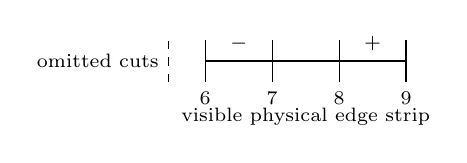
\begin{tikzpicture}[x=.85cm,y=.45cm,baseline=(current bounding box.center)]
  \foreach \x/\lab in {0/{6},1/{7},2/{8},3/{9}} {
    \draw (\x,0) -- (\x,1.2);
    \node[below] at (\x,0) {\scriptsize \(\lab\)};
  }
  \draw[thick] (0,.6) -- (3,.6);
  \node[above] at (0.5,.6) {\scriptsize \(-\)};
  \node[above] at (2.5,.6) {\scriptsize \(+\)};
  \node[below] at (1.5,-.45) {\scriptsize visible physical edge strip};
  \draw[dashed] (-.55,0) -- (-.55,1.2);
  \node[left] at (-.55,.6) {\scriptsize omitted cuts};
\end{tikzpicture}
\]
The signs in this schematic are not a full token table; they indicate the
kind of pairing used in the proof.  At a fixed local level, interior visible
endpoints pair across the strip.  An unpaired endpoint could only occur at a
deleted cut next to an omitted column.

\smallskip
\noindent\emph{Step 5: omitted-edge overflow rules out hidden endpoints.}
An unpaired reduced endpoint could only be next to a deleted cut adjacent to
some omitted column \(0<h<k\).  Such an endpoint at local level \(\lambda\)
would require
\[
  1\le \lambda\le \mu_h+1.
  \tag{4}
\]
Indeed, if \(\mu_h\ge0\), the hidden stack above \(h\) has integer levels
\(0,\ldots,\mu_h\), corresponding to local levels
\(1,\ldots,\mu_h+1\).  If \(\mu_h<0\), there is no positive local level at the
hidden cut.

But omitted-edge overflow gives \(\mu_h<0\) for every omitted column
\(0<h<k\).  Hence no positive \(\lambda\) can satisfy (4).  There are no
unpaired endpoints at deleted cuts, so all reduced endpoints are paired with
opposite-signed partners.  Therefore
\[
  \omega(B)=\omega(\partial B)=0.
\]
Combining this with (1) proves the displayed boundary/suffix cancellation.
\end{proof}

\begin{example}[A compact \(13/10\) boundary/suffix cancellation]
For the \(13/10\) example
\[
  Q=(0,1,2,3,5,6,7,6,7,8),\qquad
  Q'=(0,1,2,3,5,6,7,9,6,7),
\]
the selected suffix is \(K=I_7=\{7,8,9\}\), and the boundary row is
\(b=6\).  The total deficit is unchanged:
\[
  \defc(Q)=4=\defc(Q').
\]
The only nonzero row changes in the boundary/suffix block are
\[
  \Delta\defc_6=-1,\qquad \Delta\defc_8=+1.
\]
Thus the cancellation is visible at the row level: the boundary row loses one
unit and a suffix-internal row gains one unit.  The proof above explains why,
in general, these row-level changes can be paired after rewriting them as
signed endpoints along the physical edge list.
\end{example}

\section{The theorem}

\begin{theorem}[Deficit preservation for the NRCM]
Let \(Q\) be a valid rational position-coordinate path for coprime positive
integers \(r,s\).  If \(\NRCM(Q)\) is defined, then
\[
  \defc(\NRCM(Q))=\defc(Q).
\]
\end{theorem}

\begin{proof}
Let \(Q'=\NRCM(Q)\), and let \(K=I_k\) be the suffix selected by the NRCM.
By definition of the NRCM, \(Q'\) is valid.

The deficit is the sum of the row contributions \(\defc_i\).  Rows
\[
  1,\ldots,k-2
\]
are prefix rows, empty if \(k=1\), and their total change is zero by the
prefix-row lemma.

The only remaining rows are the boundary row \(k-1\), if it appears in the
deficit sum, and the rows inside the moved suffix \(K\).  Their total change is
zero by boundary and suffix cancellation.

These two groups partition all row contributions in
\(\defc(Q')-\defc(Q)\).  Therefore
\[
  \defc(Q')=\defc(Q).
\]
\end{proof}

\end{document}
